\section{Approach Overview}
\label{approach}

The main objective of our approach is to automatically transform an existing DSL specification (cf. upper left part in Fig.~\ref{fig:overview}) initially used to drive the development of a comprehensive integrated development environment (cf. lower left part in Fig.~\ref{fig:overview}), into a new one (cf. upper right part in Fig.~\ref{fig:overview}) that can be used to automate the development of interactive computer programming environments (cf. lower right part in Fig.~\ref{fig:overview}). 
%
% the following: from an input that contains the syntax and the operational semantics of a language defined using the Interpreter pattern enriched with a set of metadata used to configure the transformation function, our approach generates a language specialized for REPL execution (Figure~\ref{fig:overview}).
%
\begin{figure*}[htb]
	\centering
	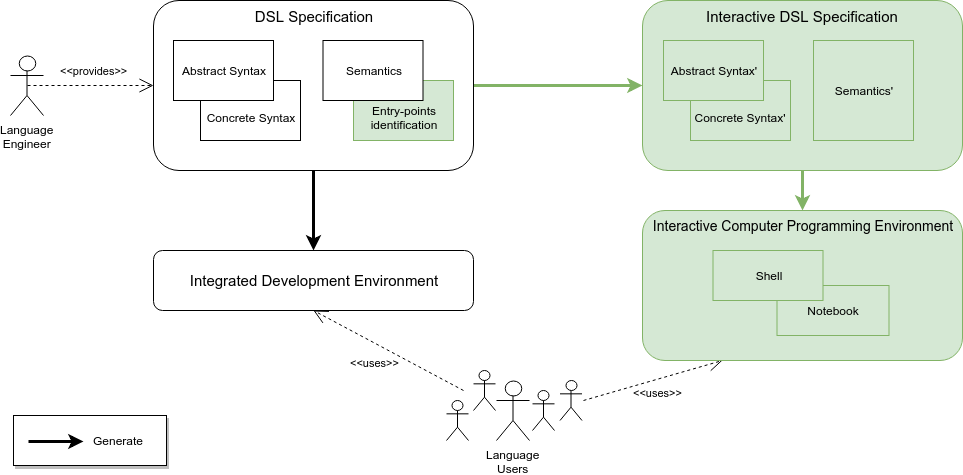
\includegraphics[width=0.7\linewidth]{figures/sle_overview.png}
	\caption{Programming environment generation from DSL specifications}
	\label{fig:overview}
\end{figure*}
%

Since we are aiming for a systematic transformation process, we put some restrictions on the supported DSLs: they need an extended BNF grammar and operational semantics that follow a pure interpreter pattern.
We believe that these characteristics are ones of the most common, and thus that these are acceptable limitations.

To reach this objective and address the RQ specified in the previous section, we identified four challenges:
\begin{itemize}
\item[C1] Identification of the different execution entry points that are meaningful for the corresponding REPL, and the expected outputs and help messages given to the user. 
\item[C2] Transformation of the syntax so that we can parse and load partial programs corresponding to the identified execution entry points. 
\item[C3] Definition of a sound yet flexible execution context and flow management,
\item[C4] Transformation of the semantics so that we can execute pieces of code corresponding to the identified execution entry points.
\end{itemize}



%\textbf{C2} How to integrate specific REPL features described at the end of section~\ref{motiv}, for example the fact that variables are set for the input expressions and results. 
%\textbf{C3} How to transform operational semantics, \emph{aka} the interpreter and its context of execution in order to allow a correct execution from all these entry points? 

%We want to obtain a complete interactive environment.
%This means two things:
%\begin{itemize}
%    \item We want the language's syntax to offer several different entry-points that are not just a complete program
%    \item The environment needs to execute the instructions inputted by the user in the same context
%\end{itemize}

% ce paragraphe doit apparaitre avant car les question de recherche ont déjà fait le choix. 

%From our experience in the field, we made the assumption that most DSLs only offer a single entry-point: a program.
%In an interactive environment however, a language user would want to have access to single statements, or even expressions, without the need to write a perfectly valid program along with it.
%To be more straightforward: a user would prefer to be able to print the value of an existing variable without having to define a class and a method when interacting with a \textit{Java} environment.
%If we take into account the fact that the language parser will not allow anything that is not a complete program, there are only two possible solutions:
%\begin{itemize}
%    \item We take the user input and add the necessary structure around it to make it an actual program
%    \item We change the language syntax to also allow non complete programs to exist
%\end{itemize}
%By using the first solution, we would then end up with a program we could execute without doing anything further.
%But this execution would quickly be out of our control, since a lot more elements than just the instruction would be included.
%We could also use the complete program only for parsing purposes and have an execution based on only the instruction, but we also need to consider how to manage the potential references to previous instructions.
%As such, we chose the second solution that gives us way more control on the process as a whole, and we can even think of reusing the grammar's validation checkers.
%%%%%%%%%%%%%%%%%%%%%%%%%%


%%%
\paragraph{Entry-points Identification (C1)}

We define as language entry-points the constructs that a language user can use and that can be executed outside of any other context.
With most traditional DSLs, the execution can only handle a complete program and builds a context for it, that will later be used by all the statements and expressions.
The only entry-point is as such the \textit{complete program}.
Here, we want to provide several entry-points with a granularity lower than a regular program.

However, the granularity of the new execution entry-points cannot be inferred automatically. The choice is up to the language engineer. In practice, they correspond to any expression to be considered as an executable statement within the interactive environment. It is therefore necessary to provide within our approach means of specifying these new entry points, and the underlying framework for loading and saving single statements. 

To report the execution entry-points, relevant abstractions must be provided to the language engineer for enhancing the initial DSL specification. Abstractions must support the identification of the relevant statements to be executed independently. Moreover, to give intermediate feedback to the language user, the new entry-points need to be also supplied with additional information about the expected outputs (\emph{e.g.,} the user would expect to get an evaluation result when he inputs a \textit{Logo} expression), and possibly an help message. 

In addition to the identification of the new execution entry-points in the DSL specification, a corresponding framework must be provided to save and load partial programs corresponding to the possible entry-points.  For such a purpose, we transform the syntax specification in order to make partial programs valid for the parser and the corresponding syntax tree.
We refer to these partial programs as \textit{instructions}.

\begin{comment}
To actually parse these new entry points, there are two possible solutions:
\begin{itemize}
   \item Complementing the user input with the required structural elements to transform an entry point in a valid program regarding the DSL specifications.
   \item To transform the language syntax specification to also allow non complete programs to be valid
\end{itemize}
By using the first solution, we would then end up with a program we could execute without doing anything further. But this execution would quickly be out of our control, since a lot more elements than just the instruction would be included.
We could also use the complete program only for parsing purposes and have an execution based on only the instruction, but we also need to consider how to manage the potential references to previous instructions.
%As such, we chose the second solution that gives us way more control on the process as a whole, and we can even think of reusing the grammar's validation checkers.
The current approach selects the second option. 
\end{comment}


%%%
\paragraph{Transformation of the syntax (C2)}

On the basis of the identified entry-points, the existing syntax specification must be transformed to enable all of these entry-points as valid instructions. A new root rule within the grammar specification and a new root node for the AST named \emph{Interpreter} are integrated. The latter contains all the newly defined valid entry points, and possibly the definitions of additional behaviors to instrument the execution. 

%%%
\paragraph{Execution context and flow management (C3)}

We don't handle complete programs anymore but independent instructions.
In order to keep a consistent execution through the different iterations of the REPL, a global execution context and its flow along the independently executed instructions must be managed. This is the role of the proposed \textit{Interpreter}, that will instantiate a context then simply pass it to instructions before executing them. Execution results must also be stored in a specific variable, and an execution trace manager must be provided to offer a complete history. 

We propose a generic interface to interact with (sequences of) instructions, used by generic interactive computer programming environments such as a language shell and a notebook interface. 

%%%
\paragraph{Transformation of the semantics (C4)}

The last step of our approach consists in transforming the DSL semantics, so that the instructions can be executed independently, over a global context, and according to the proposed interface. In order to automate this transformation, we make several assumptions about the form of the DSL specification. In our current approach, we consider operational semantics defined according to the interpreter design pattern, \emph{i.e.} an operation associated with each node of the AST, and the same context object associated with this operation containing all the dynamic information related to the language semantics. We also assume that the context passed to each nodes can be instantiated and initialized from the \textit{Interpreter} node. If the context cannot be properly initialized on its own, we still give the ability to a language engineer to include custom rules in the semantics, but we do not try to infer them during the REPL language generation. Finally, each operation associated to a node of the syntax tree declared as an entry point must not make assumptions about the execution context other than that related to the initialization, nor about the structure of the parent nodes. We defined this property as a \textit{pure} interpreter pattern. 




%%%%%%%%%%%%%%%%%%%%%%%%%%%%%%%%%%%%%%%%%%%%%%%%%%%%%%%
%%%%%%%%%%%%%%%%%%%%%%%%%%%%%%%%%%%%%%%%%%%%%%%%%%%%%%%

%Before we can do any kind of modification to enable new entry-points, we need to know of them.





%Technically, it would also possible to attach the context directly to an instruction and pass it around during execution, but then it wouldn't exist without an instruction which doesn't make sense conceptually.

%As for the semantics, it needs to reflect the changes made in the syntax.


%The action for the interpreter is to simply pass its context to an instruction before executing it.
%This means, however, that an instruction doesn't need anything else than the interpreter's context to be executed.
%We therefore require that the semantics of an instruction are written defensively and that they do not assume the structure of the program.
%To illustrate this point: if the semantics of a statement need it to be executed from within a method (because the semantics of the method has to do an initialization before it for example), then it cannot become a valid entry-point.
%The action for an instruction is then to execute the operation from the base semantics with the expected data found in the context, and also to take care of the textual output as specified by the language designer.



%%%%%%%%%%%%%%%%%%%%%%%%%%%%%%%%%%%%%%%%%%%%%%%%%%%%%%%%%%%%%


%Our approach was built around domain specific languages defined using \textit{EMF} (Eclipse Modeling Framework) and \textit{XText}, with execution semantics implemented in \textit{ALE} \cite{leduc01}.


%This new language defines an Interpreter entry-point, that manages the context and drives the execution from the top-level, and also outlines the different instructions that will become the interactive entry-points.

%A wrapper for the \textit{ALE} execution engine (Figure~\ref{fig:engine-wrapper}) takes care of creating the \textit{Interpreter} and initializing it.
%It then parses the user input into an actual executable instruction and sets it as the current instruction of the interpreter before executing it.

%The scope of previous instructions is kept by a linked list structure in the current one.
%A custom scope provider uses it for cross references resolution.

%It is important to note that we do not support adding new rules to the concrete syntax of the base language.
%Also, we decided to use the existing grammar rules as the granularity for parsing.
%The consequence is that any instruction that could not be parsed by a rule of the base language will not be supported by the REPL language.

%As for the semantics, the instruction rules need to be executable individually, which means that instructions need to either own their complete context, or use dynamic data defined globally during the initialization of the interpreter.
